\chapter{Oscillations}

\begin{definition}
    An \vocab{oscillation} is a periodic to-and-fro motion of an object between two limits.
\end{definition}

\begin{definition}
    The \vocab{amplitude} ($x_0$) is the maximum displacement of the oscillating object from its equilibrium position.
\end{definition}

Amplitude is a scalar quantity. Its SI unit is the metre.

\begin{definition}
    The \vocab{displacement} ($x$) is the distance of the oscillating object from its equilibrium position in a stated direction.
\end{definition}

Displacement is a vector quantity. Its SI unit is the metre.

\begin{definition}
    The \vocab{period} ($t$) is the time taken for the oscillating object to undergo one complete oscillation.
\end{definition}

Period is a scalar quantity. Its SI unit is the second.

\begin{definition}
    The \vocab{frequency} ($f$) is the number of complete oscillations per unit time.
\end{definition}

Frequency is a scalar quantity. Its SI unit is the Hertz (Hz).

Frequency is the reciprocal of period. \[f = \frac1T.\]

\begin{definition}
    The \vocab{angular frequency} ($\o$) is the angle per unit time, with one completely oscillation represented as $2\pi$ rad.
\end{definition}

Angular frequency is a scalar quantity. Its SI unit is radians per second (rad s$^{-1}$).

Angular frequency is related to frequency and period via \[\o = 2\pi f = \frac{2\pi}{T}.\]

\begin{definition}
    \vocab{Phase} is an angle which gives a measure of the fraction of a cycle that has been completed by the oscillating object.
\end{definition}

Phase is a scalar quantity. Its SI unit is the radian (rad).

\begin{definition}
    The \vocab{phase difference} between two oscillations is a measure of how much one oscillation is out of step with another.
\end{definition}

Phase difference is a scalar quantity. Its SI unit is the radian (rad).

\section{Simple Harmonic Motion}

There are three types of oscillations: free, damped, and forced. We look at free oscillations first.

\begin{definition}
    \vocab{Free oscillations} refer to oscillations with no external force acting, and so have constant energy and amplitude.
\end{definition}

The displacement-time graph of a free oscillation is sinusoidal. Mathematically, we can describe the displacement $x$ with respect to time $t$ with the general equations \[x = x_0 \sin{\o t + \f} \quad \tor \quad x = x_0 \cos{\o t + \f}.\] Here, the phase of the oscillating object is $\o t + \f$.

\begin{definition}
    \vocab{Simple harmonic motion} (SHM) is the oscillatory motion of a particle whose acceleration is proportional but opposite in direction to its displacement. \[a \propto -x.\]
\end{definition}

We typically define $\o^2$ to be the constant of proportionality: \[a = -\o^2 x.\] This is known as the \vocab{defining equation} for simple harmonic motion.

\begin{proposition}
    The equations $x = x_0 \sin{\o t + \f}$ and $x = x_0 \cos{\o t + \f}$ satisfy the defining equation $a = -\o^2 x$.
\end{proposition}
\begin{proof}
    Since the two expressions are phase shifts of each other, it suffices to show that either one satisfies the defining equation. We work with $x = x_0\sin{\o t + \f}$. Indeed, one can verify that the acceleration $a$ is given by \[a = \der[2]{x}{t} = -x_0 \o^2 \sin{\o t + \f} = -\o^2 x,\] so $x = x_0 \sin{\o t + \f}$ is a solution to the defining equation for simple harmonic motion.
\end{proof}

\begin{proposition}
    Given $x = x_0 \sin{\o t + \f}$, the following equations hold: \[v = x_0 \o \cos(\o t + \f) = \pm \o \sqrt{x_0^2 - x^2} \quad \tand \quad a = -x_0 \o^2 \sin{\o t + \f} = -\o^2 w.\]
\end{proposition}
\begin{proof}
    The velocity-time, acceleration-time and acceleration-displacement equations can easily be derived by repeatedly differentiating $x = x_0 \sin{\o t + \f}$ with respect to time. We now show that the velocity-displacement equation $v = \pm \o \sqrt{x_0^2 - x^2}$ holds.

    First, observe that \[v^2 = x_0^2 \o^2 \cos[2]{\o t + \f} \quad \tand \quad x^2 \o^2 = x_0^2 \o^2 \sin[2]{\o t + \f}.\] Summing the two expressions, we obtain \[v^2 + x^2 \o^2 = x_0^2 \o^2 \implies v^2 = \o^2 \bp{x_0^2 - x^2}.\] Taking roots yields \[v = \pm \o \sqrt{x_0^2 - x^2}.\]
\end{proof}

\begin{figure}[H]
    \centering
    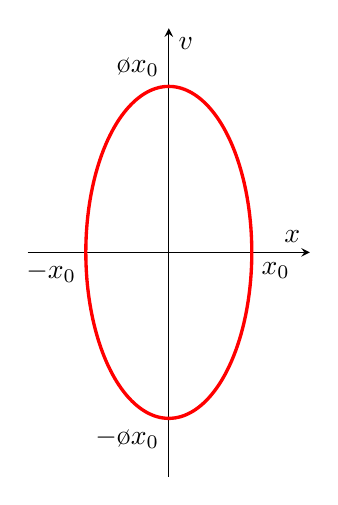
\begin{tikzpicture}[trim axis left, trim axis right]
        \begin{axis}[
            xmin = -1.7,
            xmax = 1.7,
            ymin = -2.7,
            ymax = 2.7,
            axis equal image,
            axis y line=middle,
            axis x line=middle,
            xtick = \empty,
            ytick = \empty,
            xlabel = {$x$},
            ylabel = {$v$},
            legend cell align={left},
            legend pos=outer north east,
            ]

            \addplot [domain=-2*pi:2*pi,samples=200,red, very thick]({sin(deg(x))}, {2*cos(deg(x))});
            \node[anchor=north west] at (1, 0) {$x_0$};
            \node[anchor=north east] at (-1, 0) {$-x_0$};
            \node[anchor=south east] at (0, 2) {$\o x_0$};
            \node[anchor=north east] at (0, -2) {$-\o x_0$};
        \end{axis}
    \end{tikzpicture}
    \caption{A graph of velocity against displacement.}
\end{figure}

\subsection{Energy in Simple Harmonic Motion}

\begin{proposition}
    The kinetic energy $E_k$ of a body of mass $m$ undergoing simple harmonic motion is given by \[E_k = \frac12 m \o^2 \bp{x_0^2 - x^2}.\]
\end{proposition}
\begin{proof}
    Recall that $v^2 = \o^2 \bp{x_0^2 - x^2}$, so \[E_k = \frac12 mv^2 = \frac12 m \o^2 \bp{x_0^2 - x^2}.\]
\end{proof}

\begin{corollary}
    The maximum kinetic energy is \[\max E_k = \frac12 m \o^2 x_0^2\] and occurs when $x = 0$.
\end{corollary}

Since mechanical energy is conserved, we know that \[E_{\text{total}} = E_k + E_p.\] When the kinetic energy of an oscillating object is maximum, its potential energy must be minimum. If we define $\min E_p = 0$, then \[E_{\text{total}} = \max E_k + \min E_p = \frac12 m \o^2 x_0^2.\]

\begin{proposition}
    The potential energy $E_p$ of a body undergoing simple harmonic motion is given by $\frac12 m \o^2 x^2$.
\end{proposition}
\begin{proof}
    We have \[E_p = E_{\text{total}} - E_k = \frac12 m \o^2 x_0^2 - \frac12 m \o^2 \bp{x_0^2 - x^2} = \frac12 m \o^2 x^2.\]
\end{proof}

\section{Damped Oscillations}

\begin{definition}
    \vocab{Damped oscillation} occurs when there is continuous dissipation of energy to the surroundings, resulting in a decrease in the amplitude of the oscillating system over time.
\end{definition}

There are three degrees of damping.
\begin{itemize}
    \item With \vocab{light damping}, the object undergoes a number of complete oscillations with the amplitude decreasing exponentially with time.
    \item With \vocab{critical damping}, a displaced system returns to rest at its equilibrium position in the shortest possible time without oscillating.
    \item With \vocab{heavy damping}, a displaced system takes a long time to return to its equilibrium position without oscillating.
\end{itemize}

\begin{figure}[H]
    \centering
    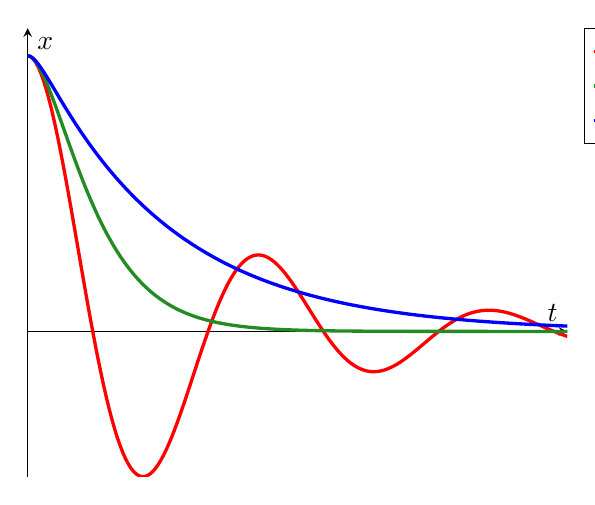
\begin{tikzpicture}[trim axis left, trim axis right]
        \begin{axis}[
            domain=0:15,
            xmax = 15,
            axis y line=middle,
            axis x line=middle,
            samples=200,
            ymax = 1.1,
            xtick = \empty,
            ytick = \empty,
            xlabel = {$t$},
            ylabel = {$x$},
            legend cell align={left},
            legend pos=outer north east,
            ]
            
            \addplot[red, very thick] {(cos(deg(0.98*x)) + 0.204*sin(deg(0.98*x))) * e^(-0.2*x)};
            \addlegendentry{Light damping};

            \addplot[ForestGreen, very thick] {(1 + x)*exp(-x)};
            \addlegendentry{Critical damping};

            \addplot[blue, very thick] {1.077*exp(-0.268*x) - 0.077*exp(-3.732*x)};
            \addlegendentry{Heavy damping};
        \end{axis}
    \end{tikzpicture}
    \caption{The displacement-time graphs of the three degrees of damping.}
\end{figure}

\section{Forced Oscillations}

\begin{definition}
    \vocab{Forced oscillations} occur when an external periodic force continuously supplies energy to an oscillating system to counteract energy lost through damping, thereby maintaining a constant amplitude of oscillation.
\end{definition}

When a system oscillates in the absence of any external force, it does so at its own \vocab{natural frequency} ($f_0$). Whatever its natural frequency, a forced oscillation takes on the frequency of the driving oscillations, called the \vocab{driving frequency}.

The amplitude of a forced oscillation varies with the driving frequency $f$.

\begin{definition}
    \vocab{Resonance} refers to the phenomenon that the oscillation amplitude reaches a maximum when the driving frequency is equal to the natural frequency of the forced oscillation.
\end{definition}

\begin{figure}[H]
    \centering
    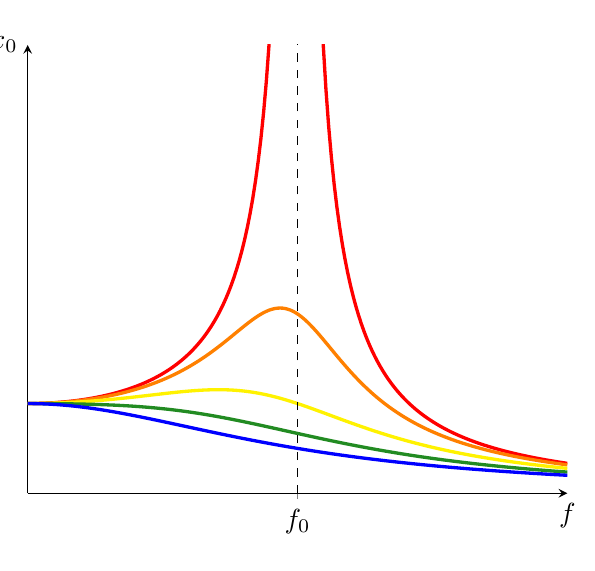
\begin{tikzpicture}[trim axis left, trim axis right]
        \begin{axis}[
            domain=0:2,
            xmax = 2,
            xmin = 0,
            ymin = 0,
            axis y line=middle,
            axis x line=middle,
            samples=200,
            ymax = 5,
            xtick = {1},
            xticklabels = {$f_0$},
            ytick = \empty,
            xlabel = {$f$},
            ylabel = {$x_0$},
            xlabel style={below},
            ylabel style={left},
            legend cell align={left},
            legend pos=outer north east,
            ]
            
            \addplot[red, very thick] {((1-x^2)^2)^(-1/2)};

            \addplot[orange, very thick] {((1-x^2)^2 + (0.5*x)^2)^(-1/2)};

            \addplot[yellow, very thick] {((1-x^2)^2 + (x)^2)^(-1/2)};

            \addplot[ForestGreen, very thick] {((1-x^2)^2 + (1.5*x)^2)^(-1/2)};

            \addplot[blue, very thick] {((1-x^2)^2 + (2*x)^2)^(-1/2)};

            \draw[dashed] (1, 0) -- (1, 10);
        \end{axis}
    \end{tikzpicture}
    \caption{Frequency response graph for varying degrees of damping. Red represents no damping, blue represents heavy damping.}
\end{figure}

As damping increases, we observe that
\begin{itemize}
    \item the response is less sharp (lower and flatter peak, and smaller amplitudes at all frequencies), and
    \item the maximum amplitude (i.e. resonance) occurs when the driving frequency is slightly less than the natural frequency.
\end{itemize}